\subsubsection{Standard Optimizations (\texttt{-O2})}
The adoption of the \texttt{-O2} optimization level leads to a moderate improvement in performance: at this level, the compiler applies \emph{conservative} optimizations that improve execution speed without "risking" changes to the program's numerical semantics or architectural meaning, such as \textbf{basic auto-vectorization}.

\begin{figure}[H]
\centering
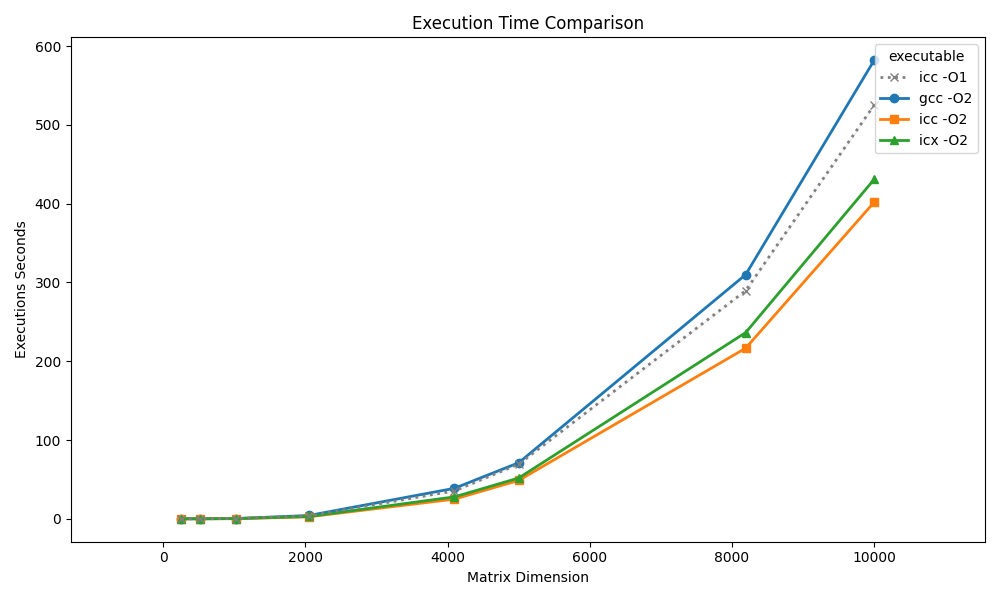
\includegraphics[width=0.8\textwidth]{Images/all_o2.png}
\caption{All compilers -O2 performances compared to ICC -O1}
\label{fig:all_o2}
\end{figure}


\paragraph{Roofline model}
The Roofline model showin in Figure~\ref{fig:icc_o2_roofline} indicates that the working point shifts vertically compared to the \texttt{-O0} configuration, reflecting increased computational throughput at similar arithmetic intensity.
Measured throughput increases to \textbf{6.062 GFLOPS}, corresponding to a 31\% improvement over the previous configuration, and execution time decreases to 49.39 seconds. 

\begin{figure}[H]
\centering
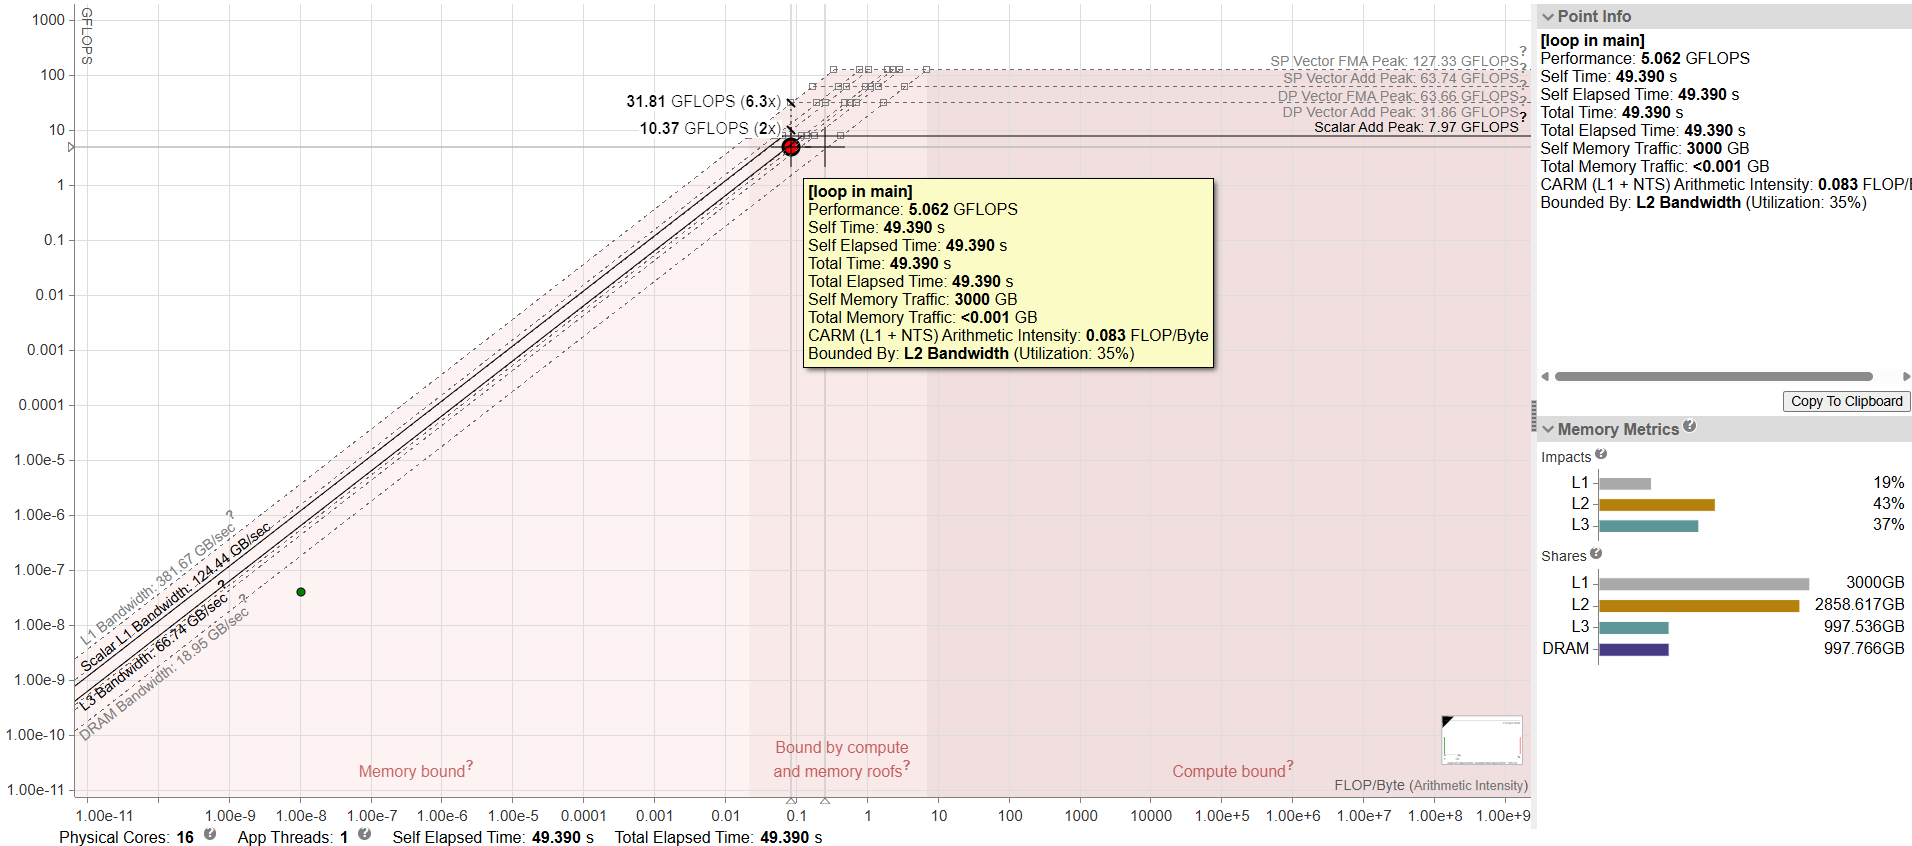
\includegraphics[width=\textwidth]{Images/icc_o2_roofline.png}
\caption{Roofline analysis for ICC -O2.}
\label{fig:icc_o2_roofline}
\end{figure}

The kernel is now bounded by L2 cache bandwidth, as explicitly reported by Advisor (``Bounded by: L2 Bandwidth''). 
This transition suggests that instruction-level inefficiencies have been partially mitigated and that the memory hierarchy has become the dominant constraint.
\paragraph{Valgrind Cachegrind Analysis.}
Dynamic analysis confirms a massive reduction in instruction overhead, though memory pressure has intensified. Key metrics are summarized in Table~\ref{tab:cachegrind_results_o2}.

\begin{table}[H]
\centering
\caption{Key Valgrind Cachegrind metrics for ICC \texttt{-O2}.}
\label{tab:cachegrind_results_o2}
\begin{tabular}{lr}
\toprule
\textbf{Metric} & \textbf{Total Count / Rate} \\
\midrule
Instruction References (I) & 297,143,584,210 \\
Data References (D)        & 187,582,341,902 \\
\midrule
L1 Data Miss Rate          & 16.7\% (25.0\% Read) \\
Last-Level (LL) Miss Rate  & 3.2\% \\
\bottomrule
\end{tabular}
\end{table}

Compared to \texttt{-O1}, the total instruction count fell by nearly 65\% (from 875B to 297B), confirming the efficacy of vectorization. However, the L1 read miss rate has spiked to 25\%. 

This occurs because the faster execution units demand data more aggressively, exposing the locality limitations of the naive $i-k-j$ pattern: the working set exceeds L2 capacity, forcing the stalls observed in the Roofline model.

\newpage
\paragraph{Compiler Report.}
The ICC optimization report confirms that the compiler successfully auto-vectorized the innermost loop, though it utilized a conservative SIMD width.

\begin{lstlisting}[style=CStyle, caption={Simplified ICC Optimization Report for \texttt{-O2}.}]
LOOP BEGIN (i-loop)
    remark #15542: loop was not vectorized: inner loop already vectorized
    LOOP BEGIN (k-loop)
        remark #15542: loop was not vectorized: inner loop already vectorized
        LOOP BEGIN (j-loop)
            remark #15388: aligned access for matrix[i][j] and matrix[k][j]
            remark #15305: vector length 2
            remark #15399: unroll factor set to 4
            remark #15300: LOOP WAS VECTORIZED
        LOOP END
        LOOP BEGIN (j-remainder)
            remark #15335: remainder loop was not vectorized
        LOOP END
    LOOP END
LOOP END
\end{lstlisting}

The report highlights a vector length of 2, indicating \texttt{\textbf{128-bit SIMD}} usage for double-precision operands. This suggests that the compiler is not yet targeting the full 256-bit register's width available on the studied AVX-capable hardware\footnote{The use of 128-bit SIMD instead of 256-bit is a symptom of the code not being fully tuned for the specific target architecture at this optimization level.}. 

Despite this, the unroll factor of 4 and aligned accesses successfully reduced loop-control overhead.
